\section{Experiments}
\label{sec:experiments}

We evaluate ApproxPilot-SE through verified hardware tradeoffs and end-to-end sample efficiency, comparing it with ApproxPilot and ApproxGNN~\cite{zhang2025approxpilot,vlcek2025approxgnn}. Mechanism-specific ablations then examine surrogate co-evolution, path-aware Delay aggregation, and local Delay calibration.


\subsection{Experimental Setup}
\label{sec:setup}

\textbf{Benchmarks and evaluation:}
The evaluation includes DCT, Laplace image filtering, Sobel edge detection, Gaussian filtering, and KMeans clustering. Table~\ref{tab:benchmarks} summarizes their arithmetic operations and configurable sites. Application quality is measured by the average Structural Similarity Index Measure (SSIM)~\cite{wang2004ssim} on the BSDS500 dataset~\cite{arbelaez2011contour} and expressed as retention relative to Exact. The arithmetic-unit library combines EvoApproxLib components and CGP-generated units; legal substitutions preserve operation type, bit width, and interface.

\begin{table}[tb]
\centering
\caption{Benchmark configurations.}
\label{tab:benchmarks}
\footnotesize
\setlength{\tabcolsep}{3pt}
\renewcommand{\arraystretch}{1.10}
\begin{tabular*}{\columnwidth}{@{\extracolsep{\fill}}llc@{}}
\toprule
Benchmark & Arithmetic operations & Configurable sites \\
\midrule
DCT & Add / Sub & 76 \\
Laplace & Add & 60 \\
Sobel & Add / Sub & 5 \\
Gaussian & Add / Mul & 17 \\
KMeans & Add / Sub / Mul / Sqrt & 16 \\
\bottomrule
\end{tabular*}
\end{table}

\textbf{Platform and baselines:}
DCT PPA labels are obtained with Synopsys Design Compiler using a 45-nm technology. ApproxPilot and ApproxGNN retain their respective model chains and search strategies, including ApproxPilot's critical-node supervision and ApproxGNN's pretrained component embeddings. Terminal PPA and SSIM are evaluated through native synthesis and application execution~\cite{zhang2025approxpilot,vlcek2025approxgnn}.

\textbf{Model training:}
The ApproxPilot-SE PPA encoder has four layers, while the SSIM encoder uses five GraphSAGE layers; both have a hidden dimension of 128. The models are trained using AdamW with a batch size of 32 for up to 120 epochs. The initial learning rates are $10^{-3}$ for PPA and $3\times10^{-4}$ for SSIM. The main DSE uses Delay-only local calibration with $d_{\max}=10$. Area, Power, and SSIM use direct predictions.

\textbf{Measurement budgets:}
ApproxPilot-SE uses 940 system-level labeled configurations, including 720 for training; each baseline uses 1060, including 900 for training.

\textbf{HV Gain:}
We report three-dimensional PPA HV Gain relative to Exact under each SSIM-retention constraint, using Exact-normalized objectives and reference point $\mathbf{r}=(1.10,1.10,1.70)$:
\begin{equation}
\mathrm{HV}_{\mathrm{Gain}}
=\mathrm{HV}(\mathcal{S}\cup\{\mathrm{Exact}\};\mathbf{r})
-\mathrm{HV}(\{\mathrm{Exact}\};\mathbf{r}),
\label{eq:hv_gain}
\end{equation}
where $\mathcal{S}$ contains the measured feasible designs.

\subsection{Overall Comparison}
\label{sec:optimization_results}

% Keep the wide result table and plots on successive pages.
\setcounter{dbltopnumber}{1}

\subsubsection{PPA Optimization Performance}

ApproxPilot-SE improves the measured PPA--quality tradeoffs on the five benchmarks. Table~\ref{tab:hv_gain} shows larger DCT HV Gain than both baselines at all five SSIM-retention thresholds. At 90\% retention, ApproxPilot-SE achieves 0.088623, compared with 0.016160 for ApproxPilot and 0.023273 for ApproxGNN. The advantage appears in the final measured designs, connecting surrogate-assisted exploration to hardware choices that satisfy the application-quality requirement. The comparison spans several quality constraints and therefore characterizes a range of operating requirements.

\begin{table*}[t]
\centering
\caption{Measured PPA HV Gain.}
\label{tab:hv_gain}
\label{tab:cross_benchmark}
\small
\setlength{\tabcolsep}{4pt}
\renewcommand{\arraystretch}{1.10}
\begin{tabular*}{0.94\textwidth}{@{\extracolsep{\fill}}llccccc@{}}
\toprule
Benchmark & Method & $\geq80\%$ & $\geq85\%$ & $\geq90\%$ & $\geq95\%$ & $\geq99\%$ \\
\midrule
\multirow{3}{*}{DCT} & ApproxPilot & 0.027075 & 0.021521 & 0.016160 & 0.000000 & 0.000000 \\
 & ApproxGNN & 0.024394 & 0.023273 & 0.023273 & 0.021611 & 0.000000 \\
 & ApproxPilot-SE & \textbf{0.101525} & \textbf{0.099683} & \textbf{0.088623} & \textbf{0.078963} & \textbf{0.064782} \\
\addlinespace[3pt]
\multirow{3}{*}{Laplace} & ApproxPilot & \textbf{0.422106} & 0.000000 & 0.000000 & 0.000000 & 0.000000 \\
 & ApproxGNN & 0.088416 & 0.088416 & 0.088416 & 0.088416 & 0.061240 \\
 & ApproxPilot-SE & 0.381159 & \textbf{0.332542} & \textbf{0.211086} & \textbf{0.144414} & \textbf{0.068019} \\
\addlinespace[3pt]
\multirow{3}{*}{Sobel} & ApproxPilot & 0.208729 & 0.133068 & 0.081493 & 0.069325 & 0.008950 \\
 & ApproxGNN & \textbf{0.229965} & 0.115541 & 0.054248 & 0.054248 & 0.009402 \\
 & ApproxPilot-SE & \textbf{0.229965} & \textbf{0.136205} & \textbf{0.096135} & \textbf{0.078954} & \textbf{0.021396} \\
\addlinespace[3pt]
\multirow{3}{*}{Gaussian} & ApproxPilot & 0.290535 & 0.236497 & 0.186049 & 0.082716 & 0.000000 \\
 & ApproxGNN & 0.295673 & 0.120928 & 0.055735 & 0.020681 & 0.004514 \\
 & ApproxPilot-SE & \textbf{0.329017} & \textbf{0.329017} & \textbf{0.243964} & \textbf{0.113170} & \textbf{0.045221} \\
\addlinespace[3pt]
\multirow{3}{*}{KMeans} & ApproxPilot & 0.377168 & 0.019913 & 0.013244 & 0.005123 & 0.000746 \\
 & ApproxGNN & 0.479862 & 0.066604 & 0.013502 & 0.013500 & 0.000000 \\
 & ApproxPilot-SE & \textbf{1.664181} & \textbf{0.663804} & \textbf{0.253267} & \textbf{0.117443} & \textbf{0.004112} \\
\bottomrule
\end{tabular*}
\end{table*}

The strict-quality region is particularly relevant when approximation must preserve the behavior of the original accelerator. At 95\% retention, the DCT HV Gain is 0.078963, compared with zero for ApproxPilot and 0.021611 for ApproxGNN. At 99\% retention, ApproxPilot-SE retains a gain of 0.064782, while both baseline design sets contribute zero additional HV beyond Exact. These results show that the proposed framework continues to identify useful hardware alternatives as the quality constraint tightens. The component analyses in Section~\ref{sec:surrogate} examine prediction, calibration, and feedback separately to explain the roles of the framework's main components.

Laplace extends the primary comparison to a filtering accelerator with a different configurable arithmetic structure. ApproxPilot-SE yields larger HV Gain than both baselines throughout the 85--99\% retention range. Its gains are 0.332542 at 85\%, 0.211086 at 90\%, 0.144414 at 95\%, and 0.068019 at 99\% retention. Table~\ref{tab:cross_benchmark} summarizes the corresponding measured gains across quality constraints. Together, the DCT and Laplace results demonstrate the framework's benefit across distinct arithmetic structures and several quality-preserving operating regions.

The additional applications broaden the comparison across edge detection, smoothing, and clustering. At 95\% retention, ApproxPilot-SE achieves HV Gains of 0.078954 on Sobel, 0.113170 on Gaussian, and 0.117443 on KMeans. On Sobel, it matches or exceeds both baselines across all five thresholds; on Gaussian and KMeans, it yields larger gains at every threshold. These comparisons establish the observed advantages within each application. All five applications retain positive ApproxPilot-SE HV Gain at the 99\% threshold, demonstrating measured hardware tradeoffs beyond Exact under a stringent quality requirement.

The design-set results translate into concrete improvements for an individual accelerator. Table~\ref{tab:representative_design} reports a DCT design that preserves 99.62\% of Exact-design SSIM while reducing area, power, and delay by 19.36\%, 20.68\%, and 9.70\%, respectively. Its mean SSIM is 0.852312, compared with 0.855541 for Exact. This example demonstrates simultaneous savings in all three hardware objectives at high output quality. It gives a practical interpretation of the design-set coverage: the measured alternatives include an implementation combining compact hardware, lower power, and shorter delay.

\begin{table}[tb]
\centering
\caption{Representative DCT design.}
\label{tab:representative_design}
\footnotesize
\renewcommand{\arraystretch}{1.12}
\setlength{\tabcolsep}{5pt}
\begin{tabular}{lccc}
\toprule
Metric & Exact & ApproxPilot-SE & Reduction \\
\midrule
Area ($\mu$m$^2$) & 3498.166 & 2820.930 & \textbf{19.36\%} \\
Power (mW) & 1.421650 & 1.127702 & \textbf{20.68\%} \\
Delay (ns) & 2.797612 & 2.526248 & \textbf{9.70\%} \\
Mean SSIM & 0.855541 & 0.852312 & -- \\
SSIM Retention & 100\% & 99.62\% & -- \\
\bottomrule
\end{tabular}
\end{table}

\subsubsection{Verified PPA--SSIM Tradeoffs}

\begin{figure*}[t]
\centering
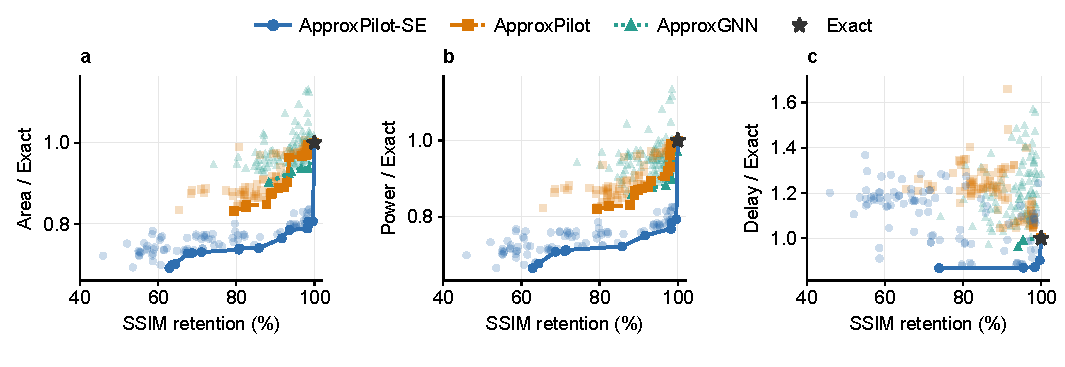
\includegraphics[width=\textwidth]{pareto_comparison.pdf}
\caption{Measured DCT PPA--SSIM tradeoffs under a matched training budget: (a) Area, (b) Power, and (c) Delay. Faint markers show verified candidates, connected markers show two-dimensional projection fronts, and stars denote Exact.}
\label{fig:measured_pareto}
\end{figure*}

Fig.~\ref{fig:measured_pareto} compares the measured DCT PPA--SSIM tradeoffs with 720 training configurations for each method. ApproxPilot-SE shifts the projected tradeoff fronts toward lower hardware costs while preserving output quality. At all five evaluated retention thresholds, it provides lower minimum Area, Power, and Delay than both baselines. Each projection minimizes one PPA objective and maximizes SSIM retention. This matched-budget view complements the joint three-dimensional PPA HV comparison in Table~\ref{tab:hv_gain}, which uses the training budgets specified in Section~\ref{sec:setup}.

Fig.~\ref{fig:output_example} compares the Exact output with that of the representative DCT design in Table~\ref{tab:representative_design}.

\begin{figure}[tb]
\centering
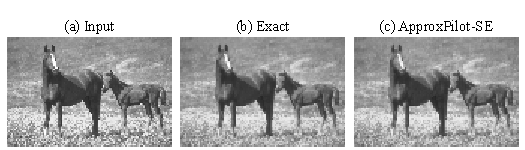
\includegraphics[width=\columnwidth]{case_113016.pdf}
\caption{Output comparison for a representative DCT design: (a) input, (b) Exact output, and (c) ApproxPilot-SE output.}
\label{fig:output_example}
\end{figure}

\subsubsection{End-to-End Sample Efficiency}
\label{sec:end_to_end_sample_efficiency}

Fig.~\ref{fig:end_to_end_sample_efficiency} evaluates end-to-end sample efficiency using the verified DCT design sets under 90\% SSIM retention. ApproxPilot-SE achieves higher HV Gain than ApproxPilot and ApproxGNN at all three training budgets. With 540 training labels, it reaches 0.079690, exceeding both baselines at 900 labels and yielding 3.42 times the gain of the stronger 900-label baseline.

\begin{figure}[!tb]
\centering
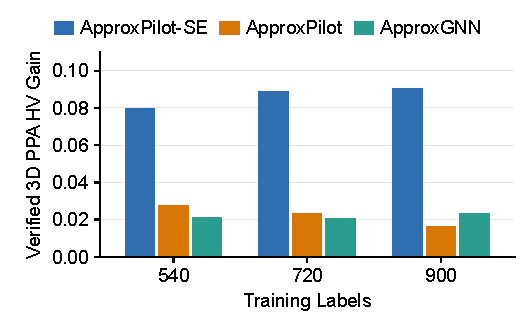
\includegraphics[width=\columnwidth]{end_to_end_sample_efficiency.pdf}
\caption{End-to-end sample efficiency on DCT under 90\% SSIM retention. All results are based on ground-truth PPA and SSIM evaluation.}
\label{fig:end_to_end_sample_efficiency}
\end{figure}

At 900 training labels, ApproxPilot-SE achieves an HV Gain of 0.090514, 3.89 times that of the strongest baseline at the same training budget. Because the metric is computed from ground-truth PPA and SSIM evaluations of terminal designs, these results demonstrate sample efficiency at the optimization level.

Table~\ref{tab:end_to_end_runtime} compares the estimated end-to-end runtimes on DCT with 720 training labels per method.

\begin{table}[tb]
\centering
\caption{End-to-end runtimes of the three methods.}
\label{tab:end_to_end_runtime}
\footnotesize
\renewcommand{\arraystretch}{1.10}
\begin{tabular}{@{}l@{\hspace{2em}}r@{}}
\toprule
Method & Time (h) \\
\midrule
ApproxPilot-SE & 4.47--6.00 \\
ApproxPilot & 4.08--5.74 \\
ApproxGNN & 5.65--8.07 \\
\bottomrule
\end{tabular}
\end{table}

\subsubsection{Surrogate Prediction Comparison}

\begin{figure*}[t]
\centering
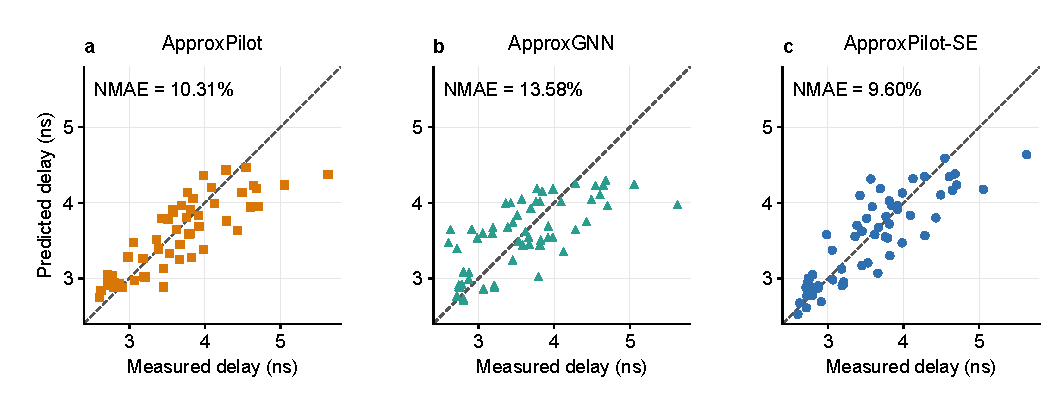
\includegraphics[width=\textwidth]{pred_vs_truth.pdf}
\caption{Delay predictions on DCT: (a) ApproxPilot, (b) ApproxGNN, and (c) ApproxPilot-SE. Dashed lines indicate ideal prediction, $y=x$.}
\label{fig:pred_vs_truth}
\end{figure*}

ApproxPilot-SE provides the lowest prediction error across all four targets in the matched 900-configuration comparison (Table~\ref{tab:surrogate_comparison}). Relative to ApproxPilot, Power and Delay NMAEs decrease by 34.9\% and 22.8\%, respectively, while SSIM MAE decreases by 31.1\%. The corresponding Spearman correlations reach 0.9412, 0.9202, and 0.9487. These metrics address two requirements of surrogate-assisted DSE: estimating the magnitude of hardware and quality changes, and preserving the relative order of candidate designs. Accurate quality prediction helps distinguish configurations near a retention constraint, while reliable PPA rankings support the selection of competitive hardware tradeoffs.

\begin{table}[tb]
\centering
\caption{Surrogate prediction performance.}
\label{tab:surrogate_comparison}
\footnotesize
\setlength{\tabcolsep}{2pt}
\renewcommand{\arraystretch}{1.10}
\begin{tabular*}{\columnwidth}
{@{\extracolsep{\fill}}llccc@{}}
\toprule
\textbf{Target} & \textbf{Metric} &
\textbf{ApproxPilot-SE} &
\textbf{ApproxPilot} &
\textbf{ApproxGNN} \\
\midrule
\multirow{2}{*}{Area}
& NMAE $\downarrow$
& \textbf{0.0130} & 0.0137 & 0.0604 \\
& Spearman $\uparrow$
& 0.9557 & \textbf{0.9625} & 0.1618 \\
\addlinespace[3pt]
\multirow{2}{*}{Power}
& NMAE $\downarrow$
& \textbf{0.0168} & 0.0257 & 0.0394 \\
& Spearman $\uparrow$
& \textbf{0.9412} & 0.8814 & 0.6014 \\
\addlinespace[3pt]
\multirow{2}{*}{Delay}
& NMAE $\downarrow$
& \textbf{0.0676} & 0.0875 & 0.1355 \\
& Spearman $\uparrow$
& \textbf{0.9202} & 0.8957 & 0.7140 \\
\addlinespace[3pt]
\multirow{2}{*}{SSIM}
& MAE $\downarrow$
& \textbf{0.0252} & 0.0366 & 0.0391 \\
& Spearman $\uparrow$
& \textbf{0.9487} & 0.9119 & 0.8925 \\
\bottomrule
\end{tabular*}
\end{table}



The Delay scatter plots in Fig.~\ref{fig:pred_vs_truth} complement this comparison at the smaller training size of 180 configurations. The methods are shown in separate panels against the same measured values. The ideal line provides a common reference for prediction residuals, while the annotations report NMAE normalized by Exact Delay. ApproxPilot-SE achieves the lowest NMAE in this comparison. The panels show prediction dispersion across the observed Delay range, which is relevant to candidate ordering and timing decisions. Both prediction comparisons use the validation set and examine surrogate behavior at different training scales.

\subsection{Ablation Studies}
\label{sec:surrogate}

We isolate the effects of surrogate co-evolution, timing-domain path aggregation, and measured-reference Delay calibration.

\subsubsection{Co-Evolution vs. One-Shot}

The one-shot control keeps the surrogate models fixed during search. Iterative feedback improves measured Pareto coverage in the 80--95\% retention region (Fig.~\ref{fig:feedback_static}). Under matched training and search budgets, HV Gain increases by 26.87\%, 27.13\%, 13.02\%, and 8.10\% at these four thresholds. The static policy provides the control for evaluating search-selected data acquisition and model updates. The endpoint is measured feasible-design coverage, connecting the feedback policy to the hardware choices ultimately available to a designer. The improvements across this quality range support using measurements acquired during exploration to update the surrogates and guide subsequent candidate selection.

\begin{figure}[tb]
\centering
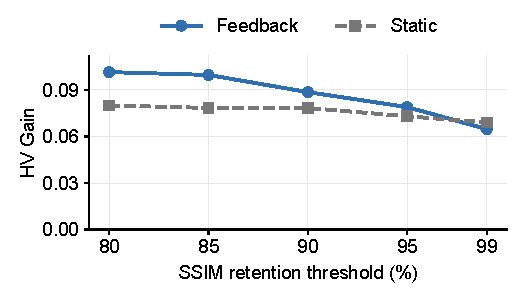
\includegraphics[width=\columnwidth]{feedback_static_hvgain.pdf}
\caption{Effect of measured feedback on DCT HV Gain.}
\label{fig:feedback_static}
\end{figure}

\subsubsection{Timing-Domain Path Aggregation}

Path-aware aggregation improves Delay prediction on the held-out set (Table~\ref{tab:delay_ablation}). Replacing global max pooling with the path-aware readout reduces mean Delay MAE by 7.45\%. Spearman correlation increases from 0.7965 to 0.8217, and pairwise ranking accuracy increases from 80.37\% to 81.67\%. The improvement appears in both numerical error and candidate ordering. In DSE, the surrogate compares configurations with different operator substitutions and must preserve useful information about their relative delays. The ablation supports incorporating graph-path dependencies into the Delay readout.

\begin{table}[!tb]
\centering
\caption{Path-aware delay readout.}
\label{tab:delay_ablation}
\footnotesize
\setlength{\tabcolsep}{5pt}
\renewcommand{\arraystretch}{1.10}
\begin{tabular}{@{}lcc@{}}
\toprule
\textbf{Metric} &
\textbf{Global Max} &
\textbf{Path-aware} \\
\midrule
MAE (ns) $\downarrow$
& $0.2095 \pm 0.0102$
& $\mathbf{0.1939 \pm 0.0022}$ \\
Spearman $\uparrow$
& $0.7965 \pm 0.0206$
& $\mathbf{0.8217 \pm 0.0228}$ \\
Pairwise Acc. (\%) $\uparrow$
& $80.37 \pm 0.88$
& $\mathbf{81.67 \pm 1.19}$ \\
\bottomrule
\end{tabular}
\end{table}

\subsubsection{Local Delay Calibration}

Measured-reference calibration improves local Delay estimates on the development set (Table~\ref{tab:local_calibration}(a)). Delay MAE decreases by 14.63\% and 17.71\% in the two training settings, accompanied by stronger Delay ranking. Calibrating SSIM affects the accuracy estimates separately; joint calibration retains the corresponding single-target improvements. DSE uses Delay-only calibration.

\begin{table}[!tb]
\centering
\caption{Local calibration analysis.}
\label{tab:local_calibration}
\label{tab:calibration_targets}
\label{tab:calibration_sensitivity}
\footnotesize
\setlength{\tabcolsep}{2pt}
\renewcommand{\arraystretch}{1.04}
\begin{tabular*}{\columnwidth}[t]{@{\extracolsep{\fill}}clccc@{}}
\toprule
\multicolumn{5}{c}{(a) Calibration targets ($d_{\max}=10$)} \\
\midrule
Labels & Targets & Delay MAE (ns) & Spearman & SSIM MAE \\
\midrule
\multirow{4}{*}{540} & Direct & 0.2404 & 0.7405 & 0.0177 \\
 & Delay & 0.2052 & 0.8040 & 0.0177 \\
 & SSIM & 0.2404 & 0.7405 & 0.0176 \\
 & Delay+SSIM & 0.2052 & 0.8040 & 0.0176 \\
\addlinespace[3pt]
\multirow{4}{*}{900} & Direct & 0.1431 & 0.8339 & 0.0182 \\
 & Delay & 0.1178 & 0.8842 & 0.0182 \\
 & SSIM & 0.1431 & 0.8339 & 0.0142 \\
 & Delay+SSIM & 0.1178 & 0.8842 & 0.0142 \\
\bottomrule
\end{tabular*}
\par\smallskip
\begin{tabular*}{\columnwidth}[t]{@{\extracolsep{\fill}}lcc@{}}
\toprule
\multicolumn{3}{c}{(b) Neighborhood sensitivity: Delay MAE (ns)} \\
\midrule
$d_{\max}$ & 540 training & 900 training \\
\midrule
Direct & 0.2404 & 0.1431 \\
0 & 0.2404 & 0.1431 \\
5 & 0.2214 & 0.1242 \\
10 & 0.2052 & 0.1178 \\
15 & 0.2082 & 0.1155 \\
20 & 0.2064 & 0.1169 \\
\bottomrule
\end{tabular*}
\end{table}

The neighborhood analysis in Table~\ref{tab:local_calibration}(b)
further demonstrates the effectiveness of local Delay calibration.
The threshold $d_{\max}=10$, selected using 540 training
configurations, is retained for the 900-configuration setting
without further tuning. Local calibration reduces Delay MAE
from 0.2404 to 0.2052 ns and from 0.1431 to 0.1178 ns,
respectively. These results demonstrate that measured
reference configurations effectively correct local prediction
biases and consistently improve Delay estimation across
different training-set sizes.

% Reserved insertion point for the unfinished feedback-batch-size study.
% \subsubsection{Feedback Batch Size}
% \label{sec:feedback_batch_size}
% Insert frozen, ground-truth-verified batch-size results when available.
% No results or conclusions are asserted by this placeholder.

\setcounter{dbltopnumber}{2}
